\section*{Aufgabe 1: \emph{Simulationskette für Netrinodetektor}}

\begin{figure}[htbp]
	\centering
	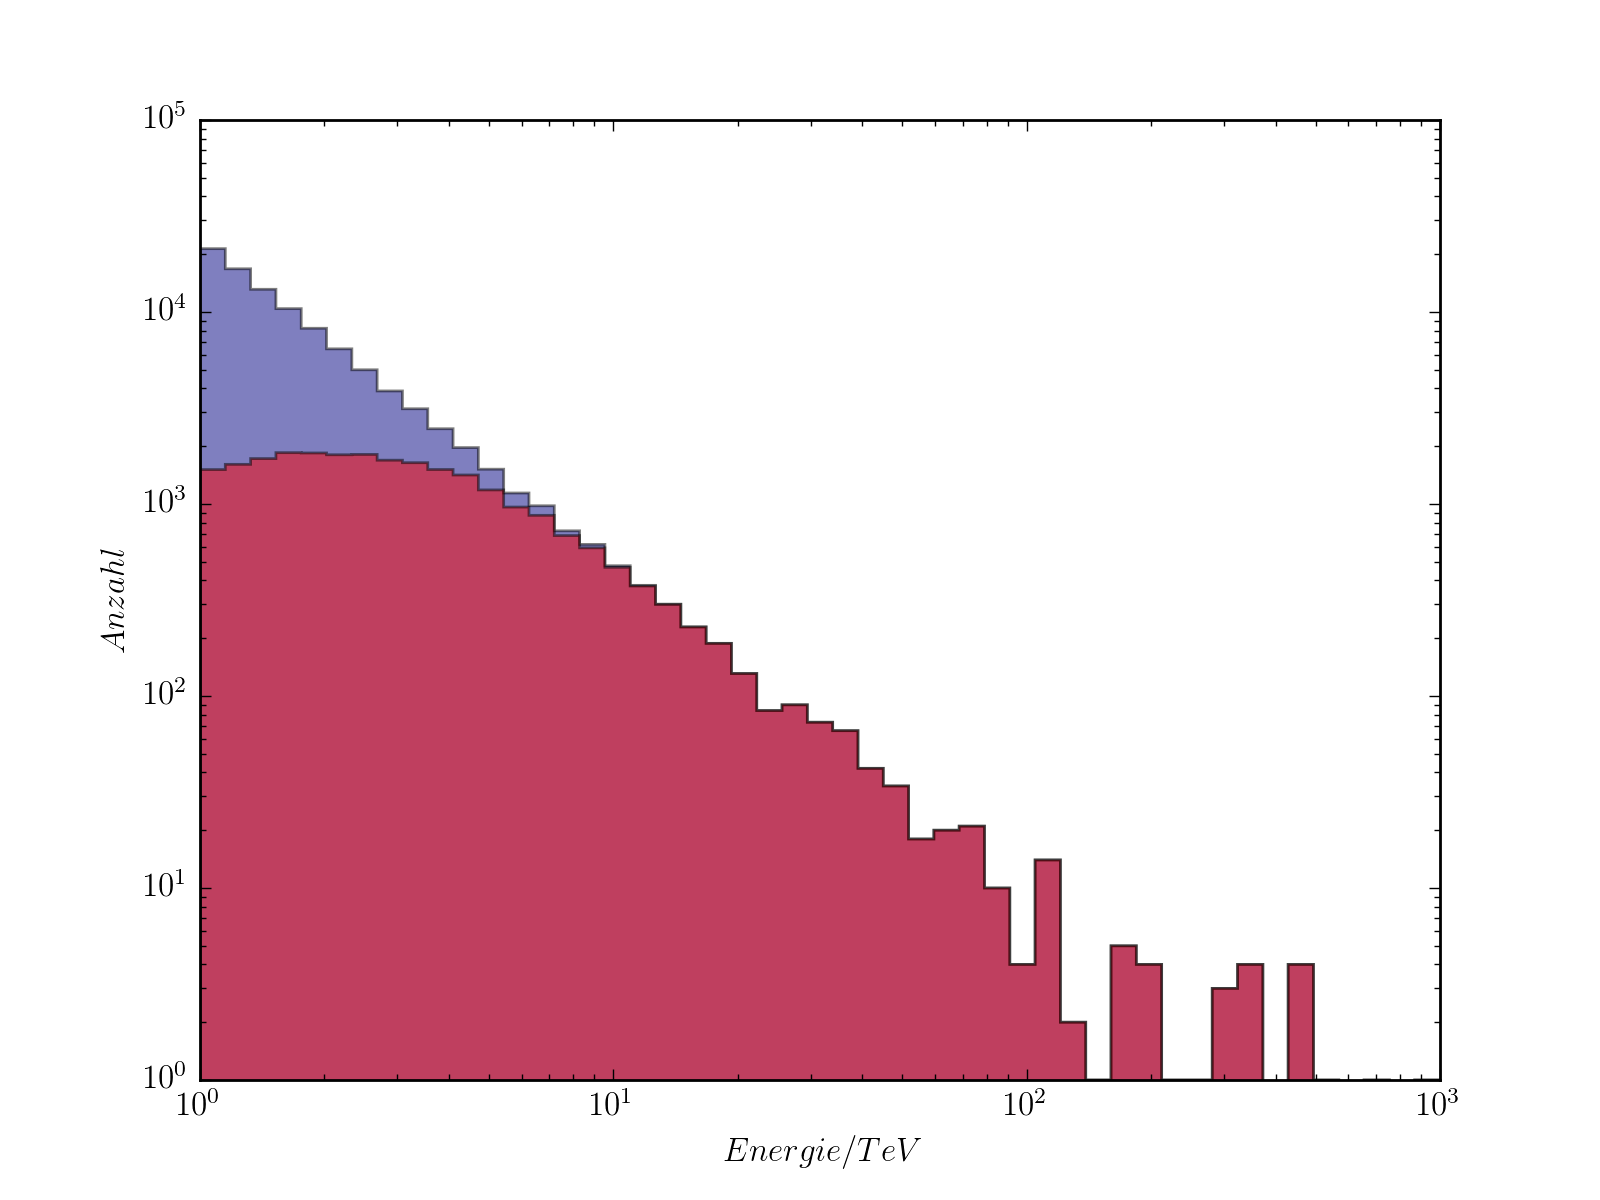
\includegraphics[width=1\textwidth]{b_hist.png}
	\caption{Histogrammierte Energien für generierte und akzeptierte Ereignisse.}
\end{figure}

\begin{figure}[htbp]
	\centering
	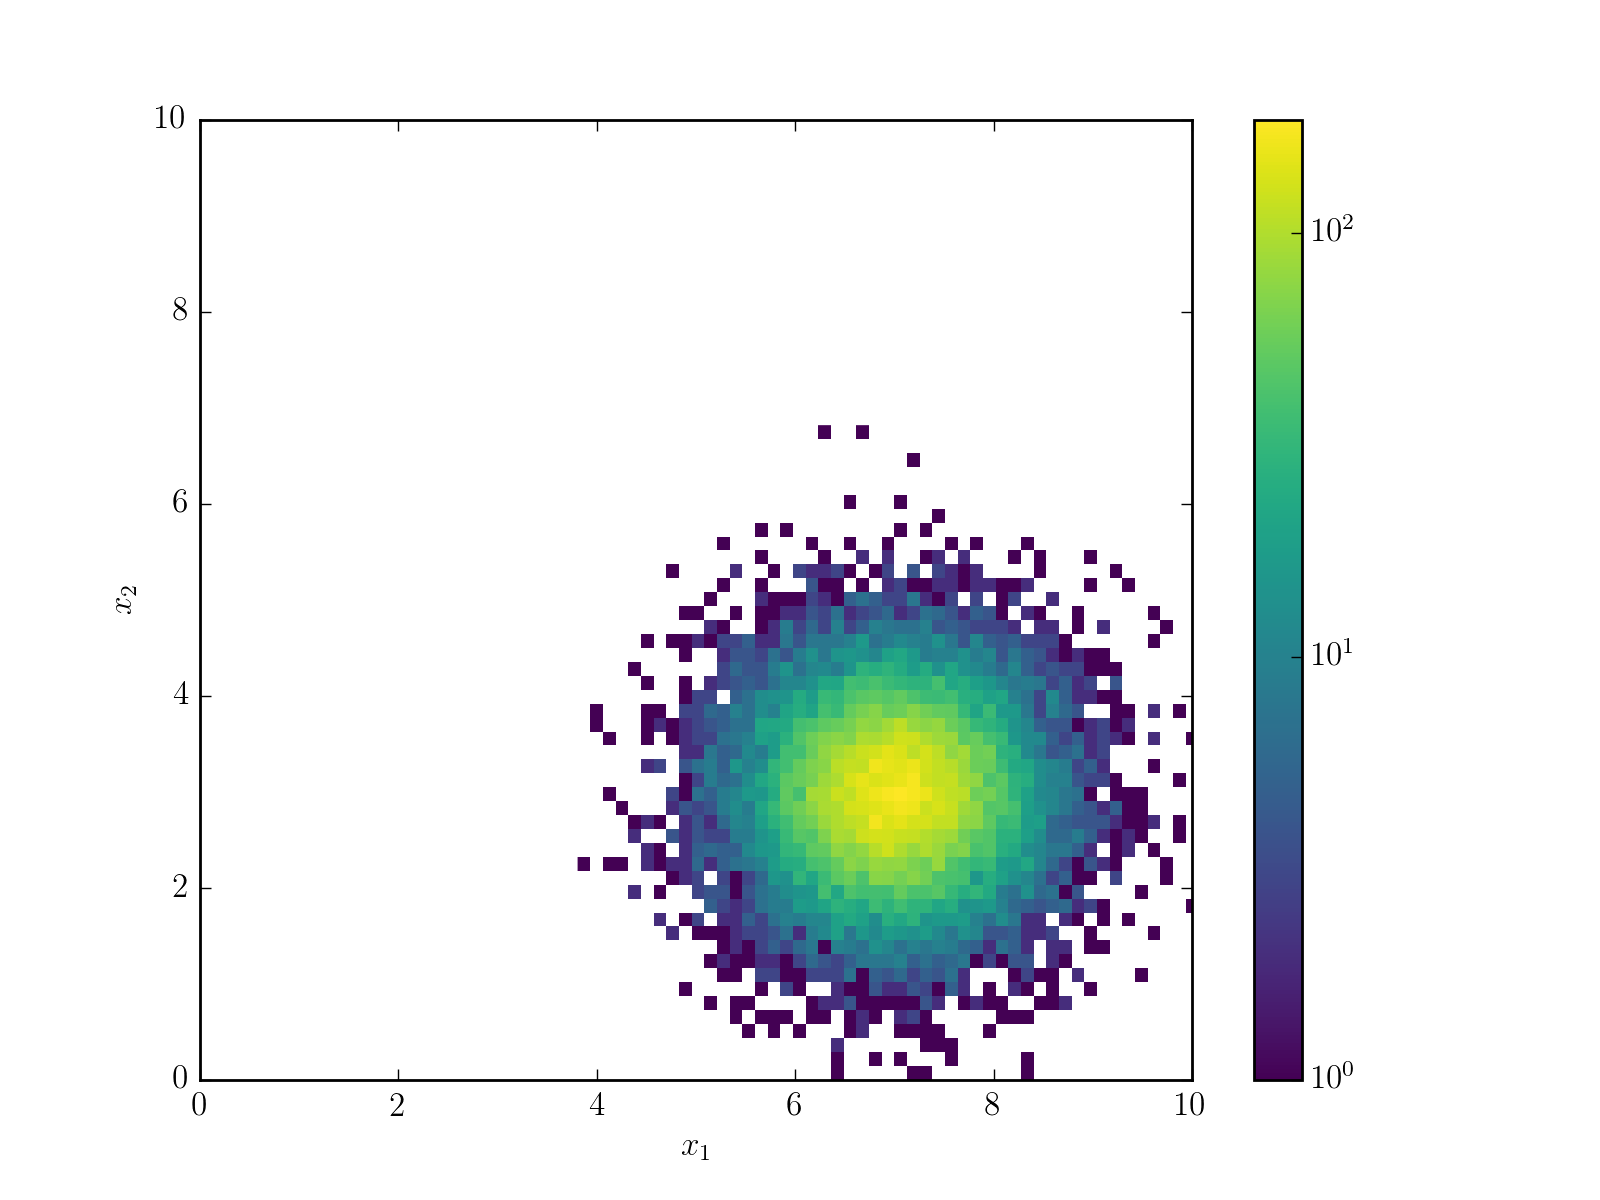
\includegraphics[width=1\textwidth]{x1_x2_hist_signal.png}
	\caption{Orte der Treffer der Signalereignisse.}
\end{figure}

\begin{figure}[htbp]
	\centering
	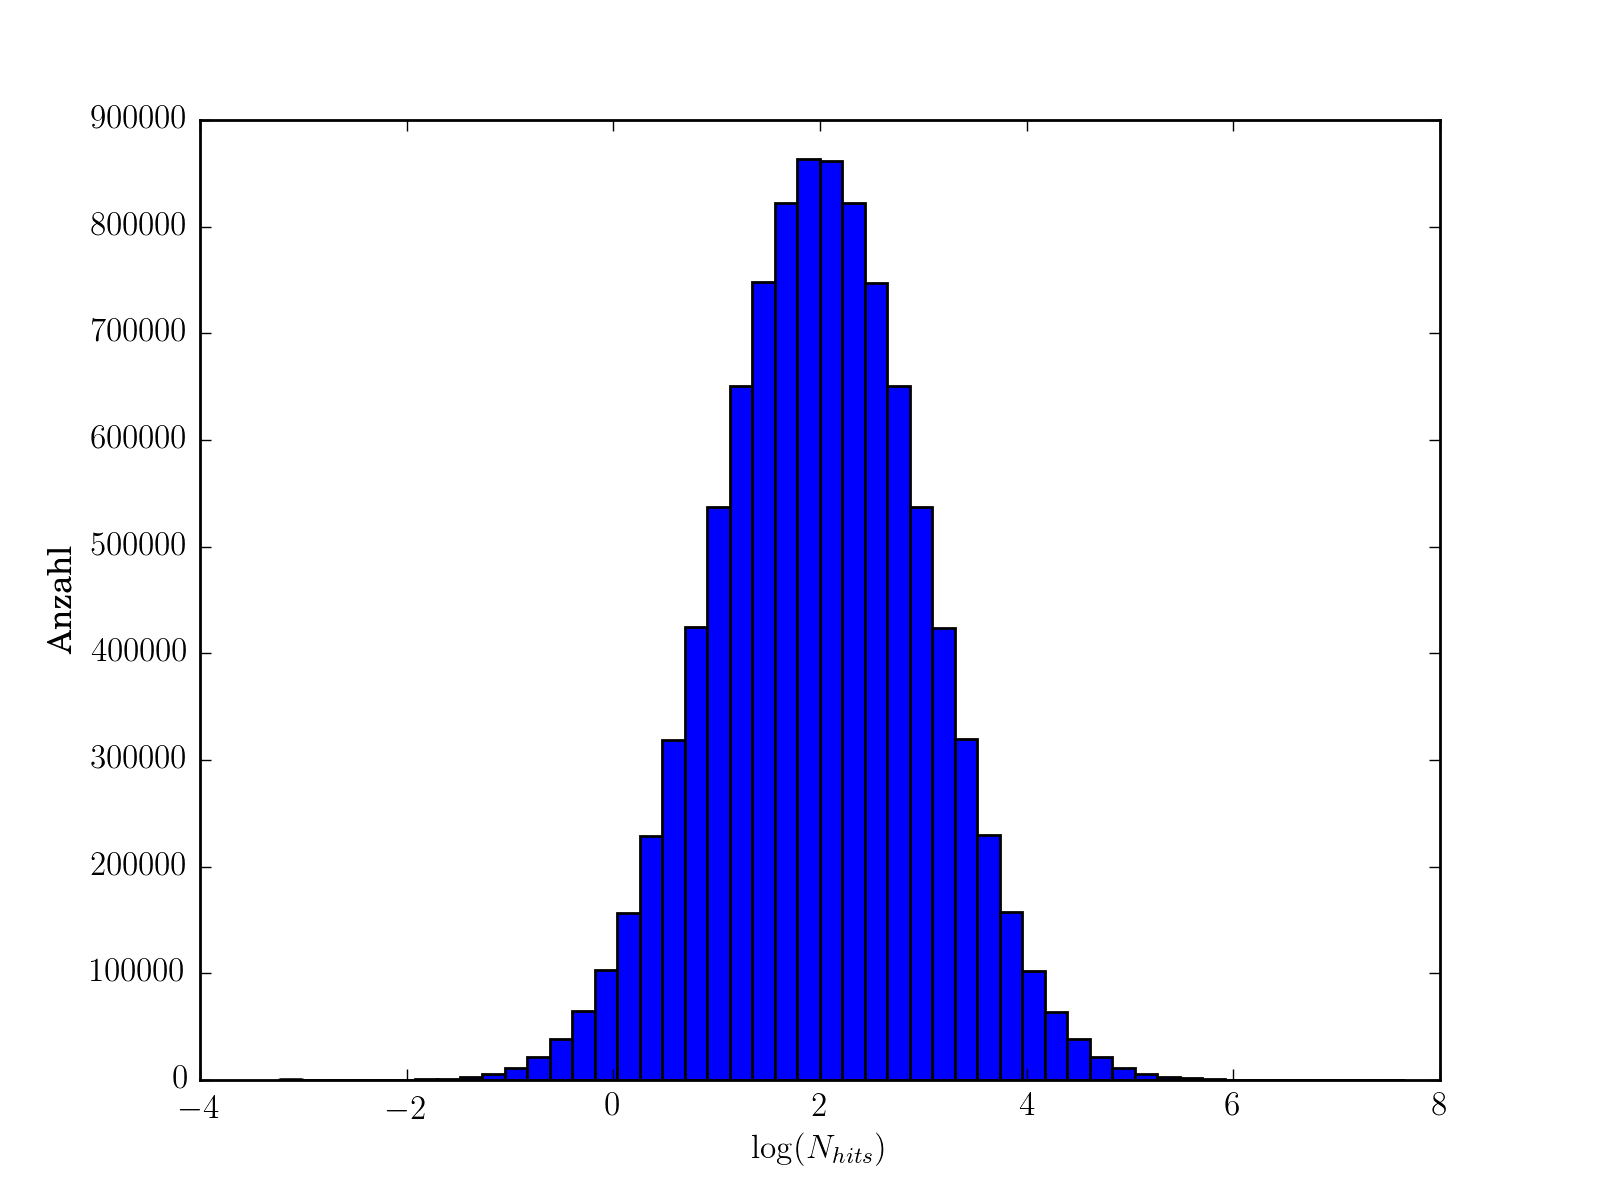
\includegraphics[width=1\textwidth]{N_hits_log.png}
	\caption{Histogramm der logartihmierten Treffer.}
\end{figure}


\begin{figure}[htbp]
	\centering
	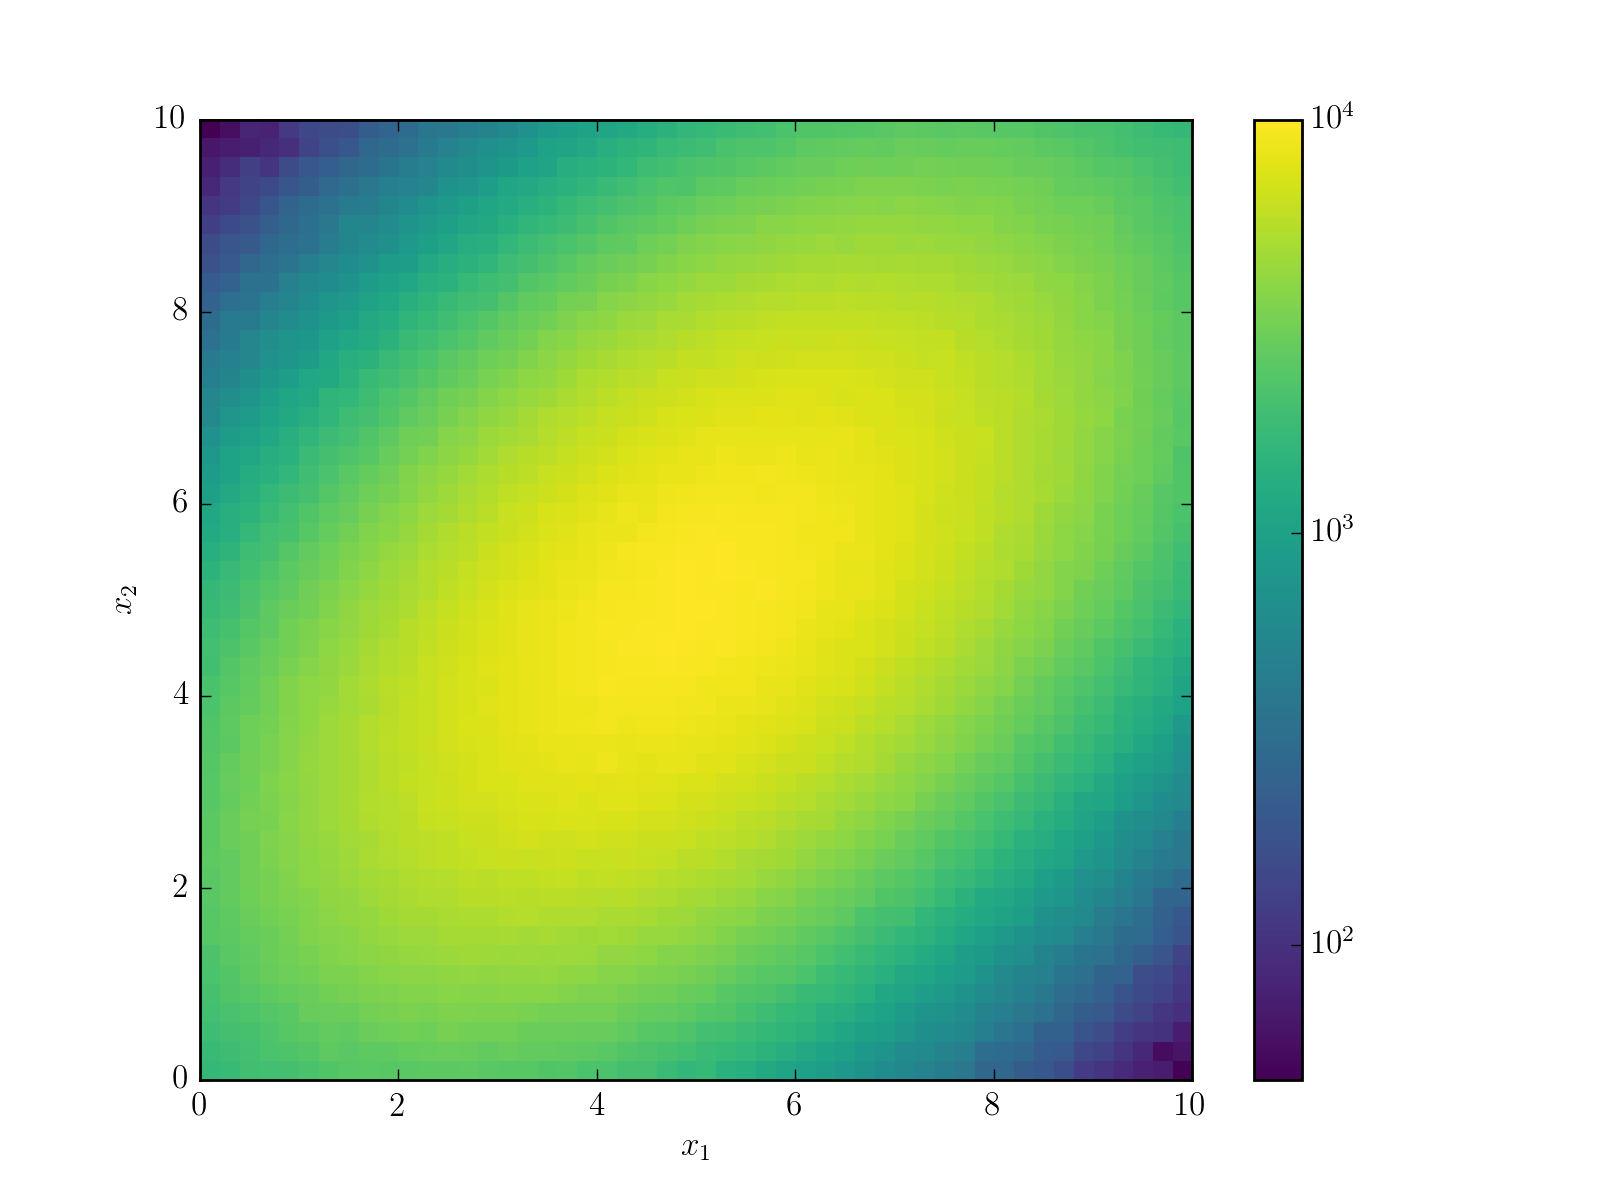
\includegraphics[width=1\textwidth]{x1_x2_hist.png}
	\caption{Orte der Treffer der Untergrundereignisse.}
\end{figure}
